\documentclass[a4paper,12pt,headsepline]{scrartcl}

%\part{title}
\usepackage[utf8]{inputenc}
\usepackage{graphicx}
\usepackage{caption,subcaption}
\usepackage[british]{babel}
\usepackage[T1]{fontenc}
\usepackage{geometry}
\usepackage{proof}
\geometry{left=3.5cm, right=2cm, top=2.5cm, bottom=2cm}
\usepackage{hyperref}
%\usepackage[hyphens,obeyspaces,spaces]{url}
\usepackage{fancybox}
\usepackage{amssymb,amsmath,amsthm}
\usepackage{gensymb}
\usepackage[linesnumbered,ruled,vlined,norelsize]{algorithm2e}
%\usepackage[bookmarksnumbered,pdftitle={\titleDocument},hyperfootnotes=false]{hyperref} 
\usepackage{color}
\usepackage{float}
\usepackage{enumerate}
\usepackage{marvosym}
\usepackage{tikz}
\usetikzlibrary{positioning}
\usetikzlibrary{patterns}
\usepackage{pgfplots}
\pgfplotsset{compat=1.12}
\usepgfplotslibrary{fillbetween}
%%%

% Always forgetting the figure parameters for precise graphical inclusions -.-

%\begin{figure}[H]
	%\centering
	%\begin{subfigure}{0.4\textwidth}
		%\centering
		%\includegraphics[width=0.34\linewidth,page=6]{includegraphics/L-%t-shape_candidates}
%		\caption{Empty $T$-face}\label{im:empty_T}	
%	\end{subfigure}
%%%
%test
%\usepackage[backend=bibtex]{biblatex}
%\usepackage{filecontents}

%\addbibresource{ref.bib}

\restylefloat{figure}

% Makros
%\newenvironment{sketch}{\begin{proof}[Proof (Sketch)]}{\end{proof}}
%\newtheorem{theorem}{Theorem}
%\newtheorem{assumption}{Assumption}
\newtheorem{lemma}{Lemma}
%\newtheorem{remark}{Remark}
%\newtheorem{definition}{Definition}
%\newtheorem{corollary}{Corollary}
\newcommand{\comment}[1]
{
  \begin{quotation}
    \textcolor{blue}{\underline{Edit:} #1}
  \end{quotation}
}
\newtheorem{aufgabe}{Exercise}
\newcommand{\Ex}[2]
{
	\setcounter{section}{#2}
	\section*{Übungsblatt #2 zu #1}
}
\newcommand{\TODO}[1]
{
  \begin{quotation}
    \textcolor{red}{\underline{TODO:} #1}
  \end{quotation}
}
% Zeichen 
\newcommand{\OO}{\ensuremath{\mathcal{O}}}
\newcommand{\ec}{\texttt{ec}}
\newcommand{\NP}{\call{NP}}
\newcommand{\call}[1]{\ensuremath{\mathcal{#1}}}

% neue Kopfzeilen mit fancypaket
\usepackage{fancyhdr} %Paket laden
\pagestyle{fancy} %eigener Seitenstil
\fancyhf{} %alle Kopf- und Fußzeilenfelder bereinigen
\fancyhead[L]{Benjamin \c Coban \\ Christoph Jabs}
\fancyhead[C]{Algorithmen und Komplexität \\ Blatt 7}
\fancyhead[R]{3526251 \\ 5567177}
\setlength{\headheight}{39pt}
\renewcommand{\headrulewidth}{0.4pt} %obere Trennlinie
%\fancyfoot[C]{\thepage} %Seitennummer
%\renewcommand{\footrulewidth}{0.4pt} %untere Trennlinie

\frenchspacing
\makeindex

% Pseudocode für Java
\usepackage{listings}
\lstset{numbers=left, numberstyle=\tiny, numbersep=5pt, keywordstyle=\color{black}\bfseries, stringstyle=\ttfamily,showstringspaces=false,basicstyle=\footnotesize,captionpos=b}
\lstset{language=java}

% Disable single lines at the start of a paragraph (Schusterjungen)
\clubpenalty = 10000
% Disable single lines at the end of a paragraph (Hurenkinder)

\widowpenalty = 10000
\displaywidowpenalty = 10000
\begin{document}
\begin{aufgabe}
\end{aufgabe}

\newpage
\begin{aufgabe}
\end{aufgabe}
The $L_1$ metrics between two points out of $\mathbb{R}^2$ is defined as:
\begin{align*}
d(p_i,p_j) = |x_i - x_j| + |y_i - y_j|
\end{align*}
\begin{enumerate}[a)]
	\item In the following figure, the rectangles along with the points of minimum distances are illustrated:
	\begin{figure}[H]
		\centering
		\begin{subfigure}{0.48\textwidth}
			\centering
			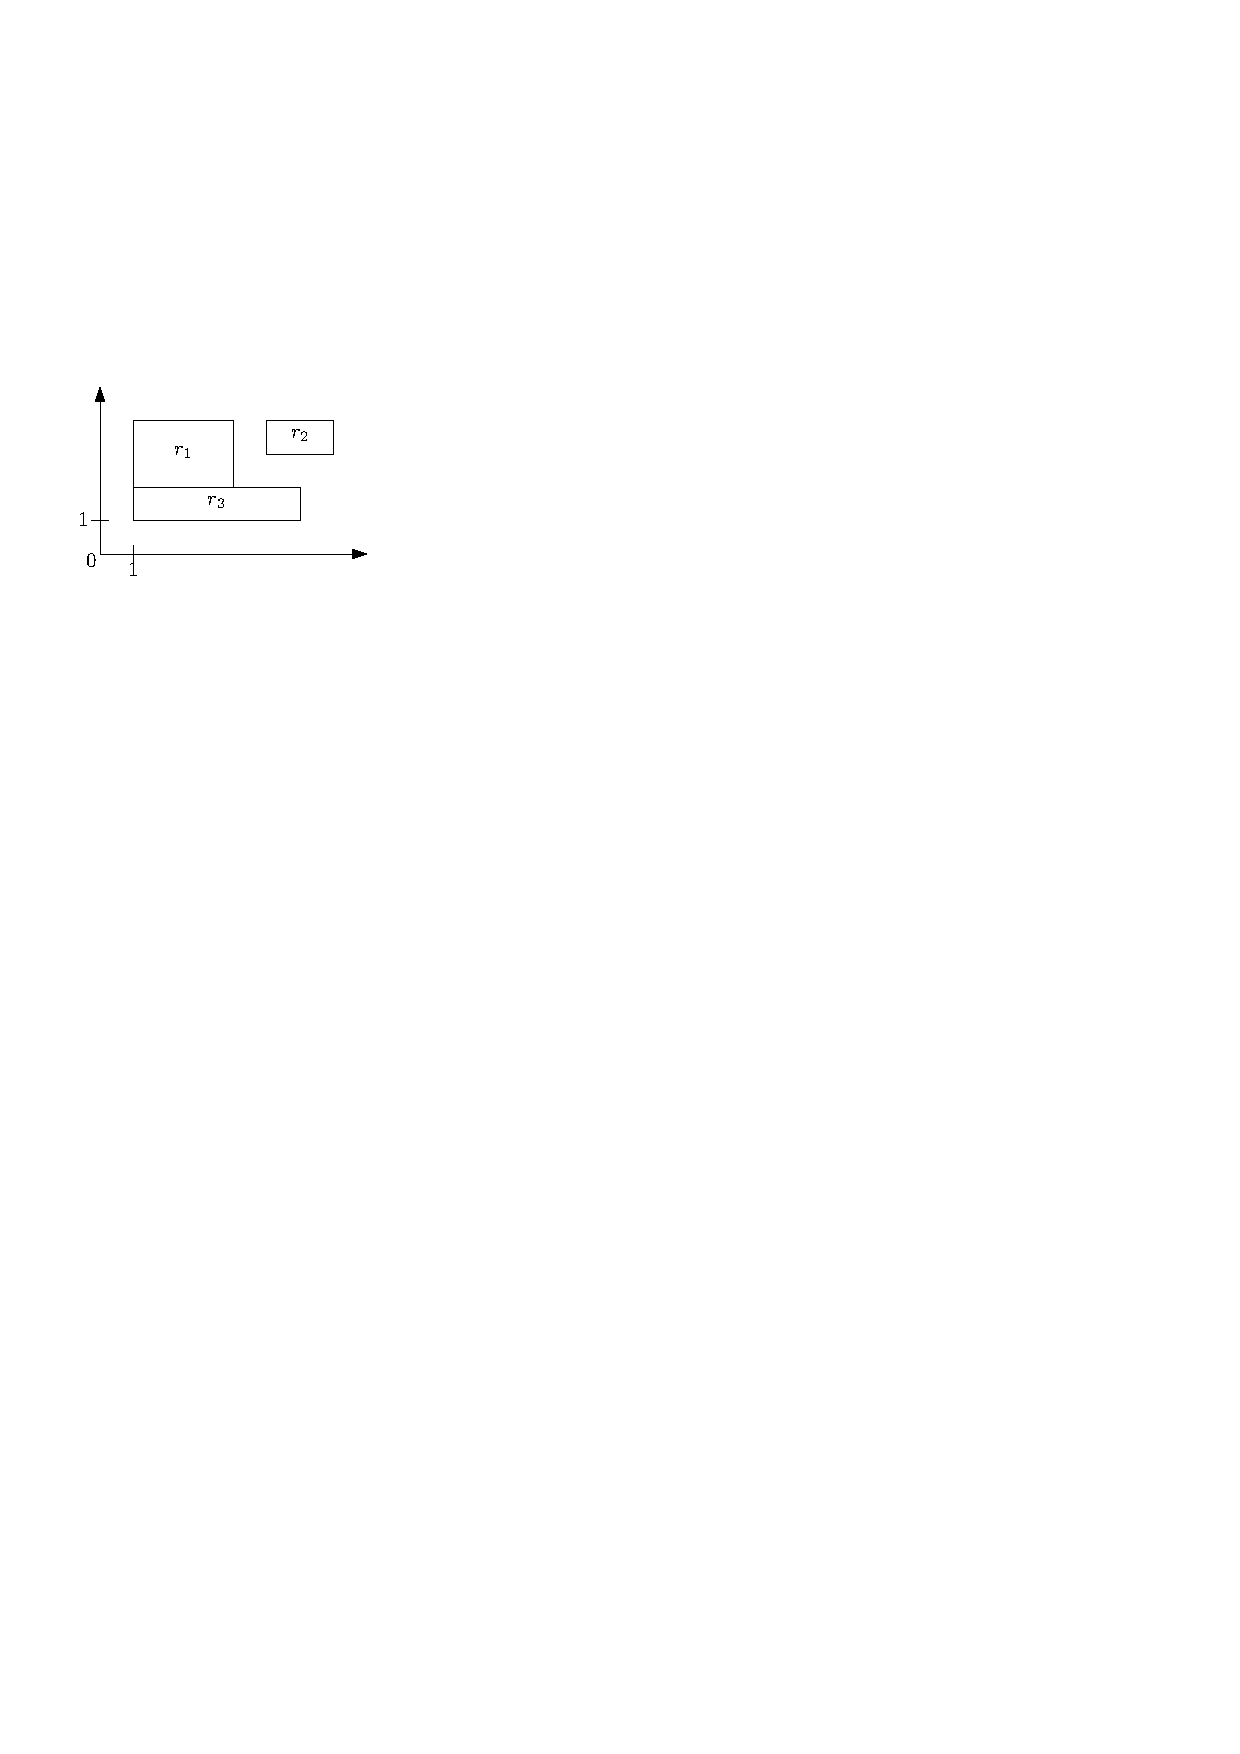
\includegraphics[width=1\linewidth,page=1]{graphics/7_2.pdf}
			\caption*{Illustration of the given rectangles}
		\end{subfigure}
		\begin{subfigure}{0.48\textwidth}
			\centering
			\includegraphics[width=1\linewidth,page=2]{graphics/7_2.pdf}
			\caption*{Solution to the given MMDPS problem}
		\end{subfigure}
	\end{figure}
An optimal solution is:
\begin{align*}
	p_1 = (4,2.5), p_2 = (5,3), p_3 = (5,2)
\end{align*}
with a diameter of 1.5.
\begin{proof}
	The minimum distance from $r_2$ to $r_1$ or $r_2$ is 1 due to the gap. To keep the distance to $r_3$ in $y$ direction and to $r_1$ in $x$ direction minimal, $p_2$ is set to the bottom left corner. Then, with two distances of 1, there is a diameter of 2 since the point set would span a square at its corners. So, the lower bound of the diameter is 1, the upper bound 2 with this approach.\\
	Next, it is to show that there is no point set with a lower diameter of 1.5. Suppose, there exists a point set $p'_1,p'_2, p'_3$ with fixed $p'_2 = p_2$ and a diameter of less than 1.5. Then, $d(p'_i,p_j') < 1.5$. Look at w.l.o.g. fixed $p'_2, p'_1$. Then, every point $p'_3$ fulfilling the diameter constraint is not in $r_3$, for all fixed points, contradicting the Minimum Manhattan Diameter Point Set.
\end{proof}
Note that this is not the only optimal solution, consider this second solution in the figure below:
	\begin{figure}[H]
	\centering
	\begin{subfigure}{0.48\textwidth}
		\centering
		\includegraphics[width=1\linewidth,page=3]{graphics/7_2.pdf}
		\caption*{Alternative solution}
	\end{subfigure}
\end{figure}
\item 
\end{enumerate}
\newpage
\begin{aufgabe}
\end{aufgabe}

\end{document}
